% a4 paper with title page on separate page
\documentclass[a4paper, titlepage]{article}
\usepackage{geometry}
\usepackage{graphicx}
\usepackage{todonotes}
% more date and time options
\usepackage{datetime}
% for only month and year in title
\newdateformat{monthyeardate}{\monthname[\THEMONTH] \THEYEAR}
% for code snippet
\usepackage{listings}
\renewcommand{\lstlistingname}{Code}
\usepackage{color}
\usepackage{float}
\usepackage[nottoc,numbib]{tocbibind}
%\usepackage{tocbibind}

% last packet to be imported
\usepackage{hyperref}

\setcounter{tocdepth}{5}
\setcounter{secnumdepth}{5}

\definecolor{codegreen}{rgb}{0,0.6,0}
\definecolor{codegray}{rgb}{0.5,0.5,0.5}
\definecolor{codepurple}{rgb}{0.58,0,0.82}
\definecolor{backcolour}{rgb}{0.95,0.95,0.92}
 
\lstdefinestyle{mystyle}{
    backgroundcolor=\color{backcolour},   
    commentstyle=\color{codegreen},
    keywordstyle=\color{magenta},
    numberstyle=\tiny\color{codegray},
    stringstyle=\color{codepurple},
    basicstyle=\footnotesize,
    breakatwhitespace=false,         
    breaklines=true,                 
    captionpos=b,                    
    keepspaces=true,                 
    numbers=left,                    
    numbersep=5pt,                  
    showspaces=false,                
    showstringspaces=false,
    showtabs=false,                  
    tabsize=2
}

\lstset{style=mystyle}

% \title{Packet Processing in Java}
% \author{Ashley Hemingway}
% \date{\monthyeardate\today}

\begin{document}

\begin{titlepage}

% Defines a new command for the horizontal lines, change thickness here
\newcommand{\HRule}{\rule{\linewidth}{0.5mm}}

% Center everything on the page
\center

\textsc{\LARGE Imperial College London}\\[1.5cm]
\textsc{\Large Individual Project}\\[0.5cm]
\textsc{\large Computing - BEng}\\[0.5cm]

\HRule \\[0.6cm]
{ \huge \bfseries Packet Processing in Java}\\[0.4cm]
\HRule \\[1.5cm]

\textsc{\LARGE Ashley Hemingway}\\[1.5cm]

\begin{minipage}{0.4\textwidth}
\begin{flushleft} \large
\emph{Supervisor:}\\
Peter \textsc{Pietzuch}
\end{flushleft}
\end{minipage}
~
\begin{minipage}{0.4\textwidth}
\begin{flushright} \large
\emph{2nd Marker:} \\
Wayne \textsc{Luk}
\end{flushright}
\end{minipage}\\[4cm]

{\large \monthyeardate\today}\\[3cm]

% Include a department/university logo - this will require the graphicx package
%\includegraphics{Logo}\\[1cm]

% Fill the rest of the page with whitespace
\vfill

\end{titlepage}

%\todo{test1}
%\todo[noline]{test2}
%\todo[inline]{test3}
%\missingfigure{test4}

\listoftodos

\newpage

\tableofcontents

\newpage

\section{Introduction}
\subsection{Motivation}
As modern computing techniques advance, people are trying to find more generic solutions to problems which have been solved by native applications in the past. A main area of focus has been network middleboxes (Figure~\ref{fig:middlebox}), which are developed to manipulate network packets. Common examples of middleboxes are firewalls, network address translators (NATs) and load balancers, all of which inspect or transform network packets in the middle of a connection between a public and private network. In recent years, people have been developing a number of programmable middleboxes which allow these generic solutions to be used on a wide scale basis.

\begin{figure}[H]
	\centering
	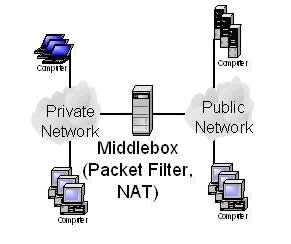
\includegraphics[scale=0.75]{images/middleboxes.jpg}
	\caption{Middlebox Example}
	\label{fig:middlebox}
\end{figure}

\noindent As middleboxes are mainly used for networking purposes, they are required to process network packets at line rate (i.e. at speeds which allow packets to be processed as they are received). This requires the application to retrieve the packet from the network line, inspect and transform the packet in the desired way and then insert the packet back onto the network line, all within a time period sufficient enough to not cause a backlog. High performance implementations of such applications are available, but are written in native languages, predominately in C/C++. However, more and more high performance computing projects are been developed in Java and have succeeded in performing at similar speeds to C/C++ applications. \\
\newline
The main challenge is actually getting the I/O system for the Java application to run at line rate speeds, due to challenges with how the JVM (Java Virtual Machine) interacts with memory and the computer's kernel. Once this challenge has been overcome, there are no reasons why programmable middleboxes written in none native languages such as Java can exist within networking systems.

\subsection{Objectives}
The main objective for this project is to research, develop and test a new application which is written in a non-native language such as Java, but can process packets at a high performance level. This also requires that the application can perform I/O operations at line rate in order to pass on data packets without slowing the line rate. The aim is to match current native applications which are written in C/C++. \\
\newline
With the main objective stated above, I set out a few initial, smaller objectives in order to divide the project into more manageable objectives:
\begin{itemize}
	\item Understand similar applications and API's written in C/C++ which process at line speeds and how the implementations can be exploited for Java applications
	\item Exploit two Java features which allows for better I/O performance: ByteBuffer's and the Java Native Interface (JNI)
	\item Implement basic middlebox applications in Java such as a firewall and a NAT
	\item Compare Java implementations to those which are pure Java and pure C/C++
\end{itemize}

\subsection{Solution Idea}
The idea is to implement a new library in Java using a few techniques in order to speed up network access. Firstly, no networking will be done via the JVM and the operating system kernel. Instead, the Java application will bypass the kernel altogether using a combination of direct memory access and high speed I/O operations via a C library which we interact with the application via the Java Native Interface (JNI). \\
\newline
This eliminates the need for the JVM to call system calls from the kernel in order to do the network access, which can be relatively slow compared to direct network access achievable from native applications.

\newpage

\section{Background}
\subsection{Network Components}
\subsubsection{Network Packets}
\todo[inline]{How packets are passed around in general}
A network packet is responsible for carrying data from a source to a destination. Packets are routed, fragmented and dropped via information stored within the packet's header. Note: in this report packets and datagrams are interchangeable. Data within the packets are generally input from the application layer, while the headers (Figure~\ref{fig:ipv4}) are generated and updated by the network layer which have a much better understanding of the protocols in use.

\begin{figure}[H]
	\centering
	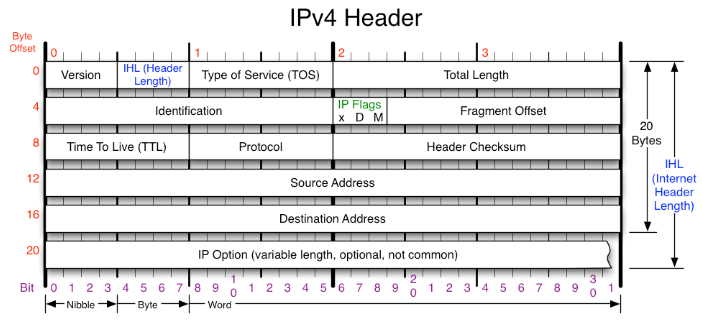
\includegraphics[width=\textwidth]{images/ipv4header.png}
	\caption{IPv4 Packet Header}
	\label{fig:ipv4}
\end{figure}

\begin{itemize}
	\item Version - IP version number (set to 4 for IPv4)
	\item Internet Header Length (IHL) - Specifies the size of the header since a IPv4 header can be of varying length
	\item Type of Service (TOS) - As of RFC 2474 redefined to be differentiated services code point (DSCP) which is used by real time data streaming services like voice over IP (VoIP) and explicit congestion notification (ECN) which allows end-to-end notification of network congestion without dropping packets
	\item Total Length - Defines the entire packet size (header + data) in bytes. Min length is 20 bytes and max length is 65,535 bytes, although datagrams may be fragmented.
	\item Identification - Used for uniquely identifying the group of fragments of a single IP datagram
	\item X Flag - Reserved, must be zero
	\item DF Flag - If set, and fragmentation is required to route the packet, then the packet will be dropped. Usually occurs when packet destination doesn't have enough resources to handle incoming packet.
	\item MF Flag - If packet isn't fragmented, flag is clear. If packet is fragmented and datagram isn't the last fragment of the packet, the flag is set.
	\item Fragment Offset - Specifies the offset of a particular fragment relative to the beginning of the original unfragmented IP datagram
	\item Time To Live (TTL) - Limits the datagrams lifetime specified in seconds. In reality, this is actually the hop count which is decremented each time the datagram is routed. This helps to stop circular routing.
	\item Protocol - Defines the protocol used the data of the datagram
	\item Header Checksum - Used for to check for errors in the header. Router calculates checksum and compares to this value, discarding if they don't match.
	\item Source Address - Sender of the packet
	\item Destination Address - Receiver of the packet
	\item Options - specifies a number of options which are applicable for each datagram. As this project doesn't concern these it won't be discussed further.
\end{itemize}

\subsubsection{Network Address Translator (NAT)}
As a routing device, a NAT is responsible for remapping an IP address to another by altering the IP datagram packet header. NAT's have become extremely important in modern networking systems due to IPv4 address exhaustion, allowing a single public IP address to map to multiple private IP addresses. This is particularly useful in large corporations where only a limited public network connection is required, meaning that all private IP addresses (usually associated with a single machine) are mapped to the same public IP address. A NAT will make use of multiple connection ports to identify which packets are for which private IP address and then re-assign the packet header so the internal routers can forward the packet correctly. As can be seen by Table~\ref{tab:ip} and Figure~\ref{fig:nat}, each internal address is mapped to via the port number associated with the external address. NAT's are generally implemented as part of a network firewall as they inspect the datagram packets for malicious data and sources.

\begin{table}[H]
	\centering
	\begin{tabular} { | c | c | }
		\hline
		\textbf{Private IP Address} & \textbf{Public IP Address} \\
		\hline
		10.0.0.1 & 14.1.23.5:62450 \\
		\hline
		10.0.0.2 & 14.1.23.5:62451 \\
		\hline
		10.0.0.3 & 14.1.23.5:62452 \\
		\hline
		10.0.0.4 & 14.1.23.5:62453 \\
		\hline
	\end{tabular}
	\caption{Example of public IP address and ports mapping to private IP address}
	\label{tab:ip}
\end{table}

\begin{figure}[H]
	\centering
	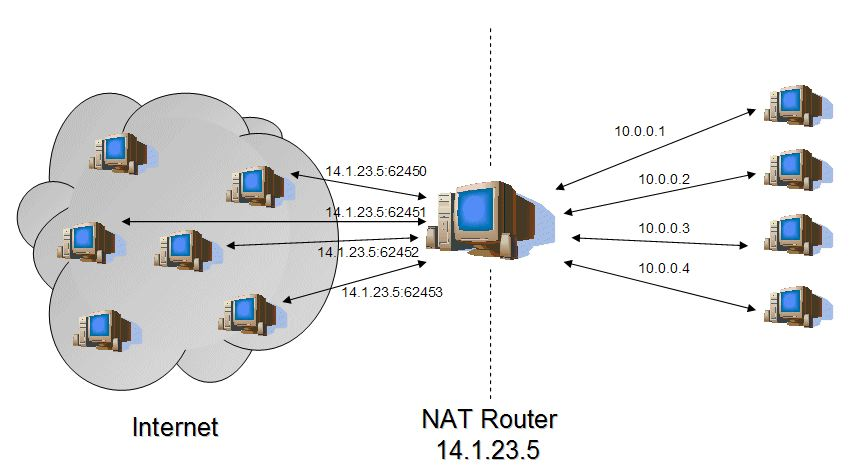
\includegraphics[width=\textwidth]{images/nat.jpg}
	\caption{NAT translating public IP addresses into private IP addresses}
	\label{fig:nat}
\end{figure}

\subsubsection{Firewall}
Firewalls (Figure~\ref{fig:firewall}) are generally the major applications which sits between the public and private network of a system. They provide packet filtering which controls which packets can enter the private network via establishing a set of rules which packets have to adhere to. Filtering can be based on a number attributes of the packet such as the source and destination IP address and port and the destination service. Firewalls can also offer a number of other useful features such as NAT's or dynamic host configuration protocol (DCHP). As well as providing protection on a network level, application layer firewalls exist which stop certain applications from sending or receiving a packet. \\
\newline
Within this project, the term 'firewall' is used for a network layer firewall which filters packets dependent on the source IP address. Any changes in this will be mentioned within the relevant sections. \\

\begin{figure}[H]
	\centering
	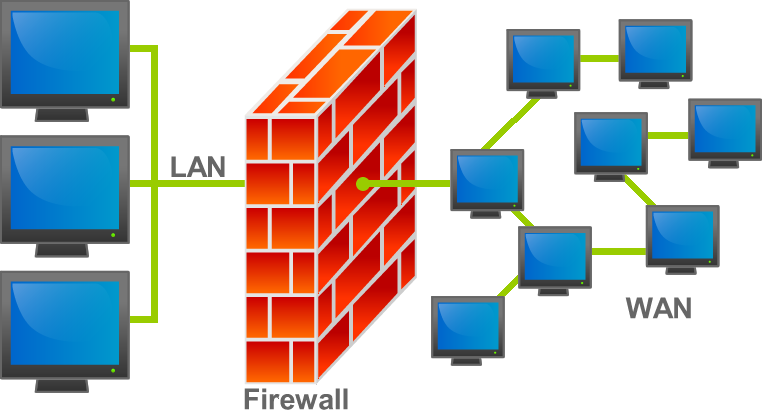
\includegraphics[width=0.7\textwidth]{images/firewall.png}
	\caption{Firewall intercepting packets to prevent security issues}
	\label{fig:firewall}
\end{figure}

\subsection{Java Features}
As the Java language and the JVM implementation is known by most, this section will focus on the more specific sections related to this project, instead of discussing the overall implementation.

\subsubsection{Java Virtual Machine (JVM)}

\begin{figure}[H]
	\centering
	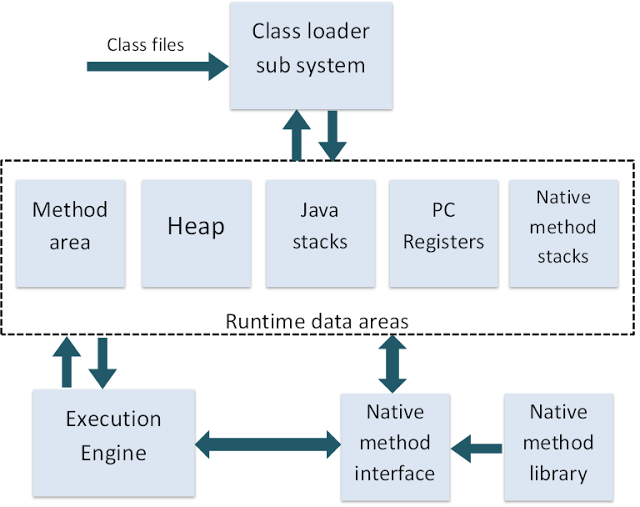
\includegraphics[width=\textwidth]{images/jvm.png}
	\caption{Java Virtual Machine interface}
	\label{fig:jvm}
\end{figure}

\begin{itemize}
	\item Class loader sub system - Loads .class files into memory, verifies byte code instructions and allows memory required for the program
	\item Method area - stores class code and method code
	\item Heap - New objects are created on the heap
	\item Stack - Where the methods are executed and contains frames where each frame executes a separate method
	\item PC registers - Program counter registers store memory address of the instruction to be executed by the micro processor
	\item Native method stack - Where the native methods are executed.
	\item Native method interface - A program that connects the native method libraries with the JVM
	\item Native method library - holds the native libraries information
	\item Execution engine - Contains the interpreter and just in time compiler (JIT - converts byte code to machine code). JVM decides which parts to be interpreted and when to use JIT compiler.
\end{itemize}

\subsubsection{Java Native Interface (JNI)}
Provided by the Java Software Development Kit (SDK), the JNI is a native programming interface that lets Java applications use libraries written in other languages. The JNI also includes the invocation API which allows a JVM to be embedded into native applications. This project and therefore this overview will only focus on Java code using C libraries via the JNI on a linux based system\\
\newline
In order to call native libraries from Java applications a number of steps have to be undertaken as shown below, which are described in more detail later:
\begin{enumerate}
	\item Java code - load the shared library, declare the native method to be called and call the method
	\item Compile Java code - compile the Java code into bytecode
	\item Create C header file - the C header file will declare the native method signature and is created automatically via a terminal call
	\item Write C code - write the corresponding C source file
	\item Create shared library - create a shared library file (.so) from C code
	\item Run Java program - run the Java program which calls the native code
\end{enumerate}

\begin{lstlisting}[language=Java, caption={Basic Java class showing native method declaration and calling with shared library loading}, label=lst:java]
public class Hello {
    public native void sayHi(String who, int times);

    static { System.loadLibrary("Hello"); }

    public static void main(String[] args) {
        Hello hello = new Hello();
        
        hello.sayHi(args[0], Integer.parseInt(args[1]));
    }
}
\end{lstlisting}

Code~\ref{lst:java} shows a simple Java program which uses some native C code from a shared library. Line 4 indicates which shared library to load into the application, which is by default lib*.so where * indicates the name of the C file. Line 2 is the native method declaration which specifies the name of the method and the parameters which will be passed to the corresponding C method. Line 9 is where this native method is called.

\begin{lstlisting}[language=sh, caption={Compiling basic Java program}, label=lst:javacomp]
$ javac Hello.java
\end{lstlisting}

Code~\ref{lst:javacomp}, run from a terminal, compiles the Java class and create a class file which can be executed.

\begin{lstlisting}[language=sh, caption={Generating C header file}, label=lst:gen]
$ javah -jni Hello.java
\end{lstlisting}

In order to generate the C header file the command 'javah' (Code~\ref{lst:gen}) is used with the flag 'jni' which tells Java that a header file is required which is for use with the JNI. It will then produce method signatures which correspond to the native method declared within Hello.java. The auto generated C header file is shown in Code~\ref{lst:auto}.
\todo[noline]{Explain parameters and mapping for jString to char* etc}

\begin{lstlisting}[language=C, caption={Auto-generated C header file}, label=lst:auto]
/* DO NOT EDIT THIS FILE - it is machine generated */
#include <jni.h>
/* Header for class Hello */

#ifndef _Included_Hello
#define _Included_Hello
#ifdef __cplusplus
extern "C" {
#endif
/*
 * Class:     Hello
 * Method:    sayHi
 * Signature: (Ljava/lang/String;I)V
 */
JNIEXPORT void JNICALL Java_Hello_sayHi
  (JNIEnv *, jobject, jstring, jint);

#ifdef __cplusplus
}
#endif
#endif
\end{lstlisting}

\begin{lstlisting}[language=C, caption={C source file corresponding to auto-generated header file}, label=lst:source]
#include <stdio.h>
#include "Hello.h"

JNIEXPORT void JNICALL Java_Hello_sayHi
(JNIEnv *env, jobject obj, jstring who, jint times) {
    jint i;
    jboolean iscopy;
    const char *name;
    name = (*env)->GetStringUTFChars(env, who, &iscopy);
    for (i = 0; i < times; i++) {
        printf("Hello %s\n", name);
    }
}
\end{lstlisting}

The C source file implementation is in Code~\ref{lst:source}. Line 9 is the interesting line, where the code is retrieving the string stored at pointer 'who' from the Java environment and copying it into the pointer 'name' for use later on.

\begin{lstlisting}[language=sh, caption={Terminal commands to generate shared library file (.so)}, label=lst:shared]
$ cc -c -I/System/Library/Frameworks/JavaVM.framework/Headers Hello.c
$ cc -dynamiclib -o libhello.so Hello.o -framework JavaVM
\end{lstlisting}

The 2 commands in Code~\ref{lst:shared} will first compile the C source code into an object file (.o), requiring a pointer to the jni.h file provided with the Java framework. The second line then generates the required shared object file (.so) which the Java application looks for.

\begin{lstlisting}[language=sh, caption={Output from running Java application calling native C methods}, label=lst:output]
$ java Hello Packet-Processing 5
Packet-Processing
Packet-Processing
Packet-Processing
Packet-Processing
Packet-Processing
\end{lstlisting}

Running the Java application with the required parameters will output the above in Code~\ref{lst:output}. \\
\newline
As can be seen in the example code (Code~\ref{lst:source}), there are 2 extra parameters in the method signature that weren't defined within the Java native method signature (Code~\ref{lst:java}). The 'env' pointer is a structure that contains the interface to the JVM, therefore providing numerous functions required to interact with the JVM and the Java objects. Examples include converting native arrays to Java arrays and throwing exceptions, allowing standard Java operations to be executed within the native C libraries via this interface. \\
\newline
The 'obj' argument refers to the Java object which the native method had been declared within. \\
\newline
Although the JNI provides a very useful interface to interact with native library code, there are a number of issues that users should be wary of before progressing:
\begin{itemize}
	\item The Java application that relies on the JNI loses its portability with the JVM as it relies on natively compiled code.
	\item Errors within the native code can potentially crash the JVM, with certain errors been very difficult to reproduce and debug.
	\item Anything instantiated with the native code won't be collected by the garbage collector with the JVM, so freeing memory should be a concern.
	\item If using the JNI on large scale, converting between Java objects and C structs can be difficult
\end{itemize}

\subsubsection{Current Java Networking Methods}
For high performance computing in Java, a number of existing programming options are available in order for applications to communicate over a network. These can be classified as: (1) Java sockets; and (2) Remote Method Invocation (RMI); (3) shared memory programming. As will be discussed, none of these are capable of truly high performance networking, especially at line rate speeds.

\paragraph{Java Sockets}\mbox{}\\ %subsubsubsection
Java sockets are the standard low level communication for applications are most networking protocols have socket implementations. They allow for streams of data to be sent between applications as a socket is one end point for a 2 way communication link, meaning that data can be read from and written to a socket in order to transfer data. Even though sockets are a viable option for networking, both of the Java socket implementations (IO sockets \& NIO (new I/O) sockets) are inefficient over high speed networks (reference here) and therefore lack the performance that is required. As discussed previously, the poor performance is due to the JVM interacting with network cards via the OS kernel.

\paragraph{Remote Method Invocation (RMI)}\mbox{}\\ %subsubsubsection
\label{subsec:rmi}
Remote Method Invocation (RMI) is a protocol developed by Java which allows an object running in a JVM to invoke methods on another object running on a different JVM. Although this method provides a relatively easy interface for which JVM's can communicate, its major drawback relates to the speed. Since RMI uses Java sockets as its basic level communication method, it faces the same performance issues as mentioned in section~\ref{subsec:rmi}.

\paragraph{Shared Memory Programming}\mbox{}\\ %subsubsubsection
Shared memory programming provides high performance JVM interaction due to Java's multithread and parallel programming support. This allows different JVM's to communicate via objects within memory which is shared between the JVM's. However, this technique requires the JVM's to be on the same shared memory system, which is a major drawback for distributed systems as scalability options decrease. \\

Even though these 3 techniques allow for communication between JVM's, the major issue is that incoming packets are still handled by the kernel and then passed onto the corresponding JVM. This means that packets are destined for certain applications, meaning that generic packets can't be intercepted and checked, which is a requirement for generic middlebox software. There is also the issue that all packets are processed via the kernel, which is a major speed reducer which limits the line rate.

\subsection{jVerbs}
Ultra-low latency for Java applications has been partially solved by the jVerbs (reference) framework. Using remote direct memory access (RDMA), jVerbs provides an interface for which Java applications can communicate, mainly useful within large scale data centre applications. \\
\newline
RDMA is a technology that allows computers within a network to transfer data between each other via direct memory operations, without involving the processor, cache or operating system of either communicating computer. RDMA implements a transport protocol directly within the network interface card (NIC), allowing for zero copy networking, which allows a computer to read from another computer and write to its own direct main memory without intermediate copies. High throughput and performance is a feature of RDMA due to the lack of kernel involvement, but the major downside is that it requires specific hardware which supports the RDMA protocol, while also requiring the need for specific computer connections set up by sockets. \\
\newline
As jVerbs takes advantage of mapping the network device directly into the JVM, bypassing both the JVM and operating system (Figure~\ref{fig:jverb}), it can significantly reduce the latency. In order to have low level interaction with the NIC, jVerbs has a very thin layer of JNI calls which can increase the overhead slightly. However, jVerbs is flawed, mainly because it requires specific hardware to run on, firstly limited by the RDMA protocol reliant hardware and further by the required RDMA wrappers which are implemented by the creators. Also, it can only be used for specific computer to computer connection and not generally packet inspection. 

\begin{figure}[H]
	\centering
	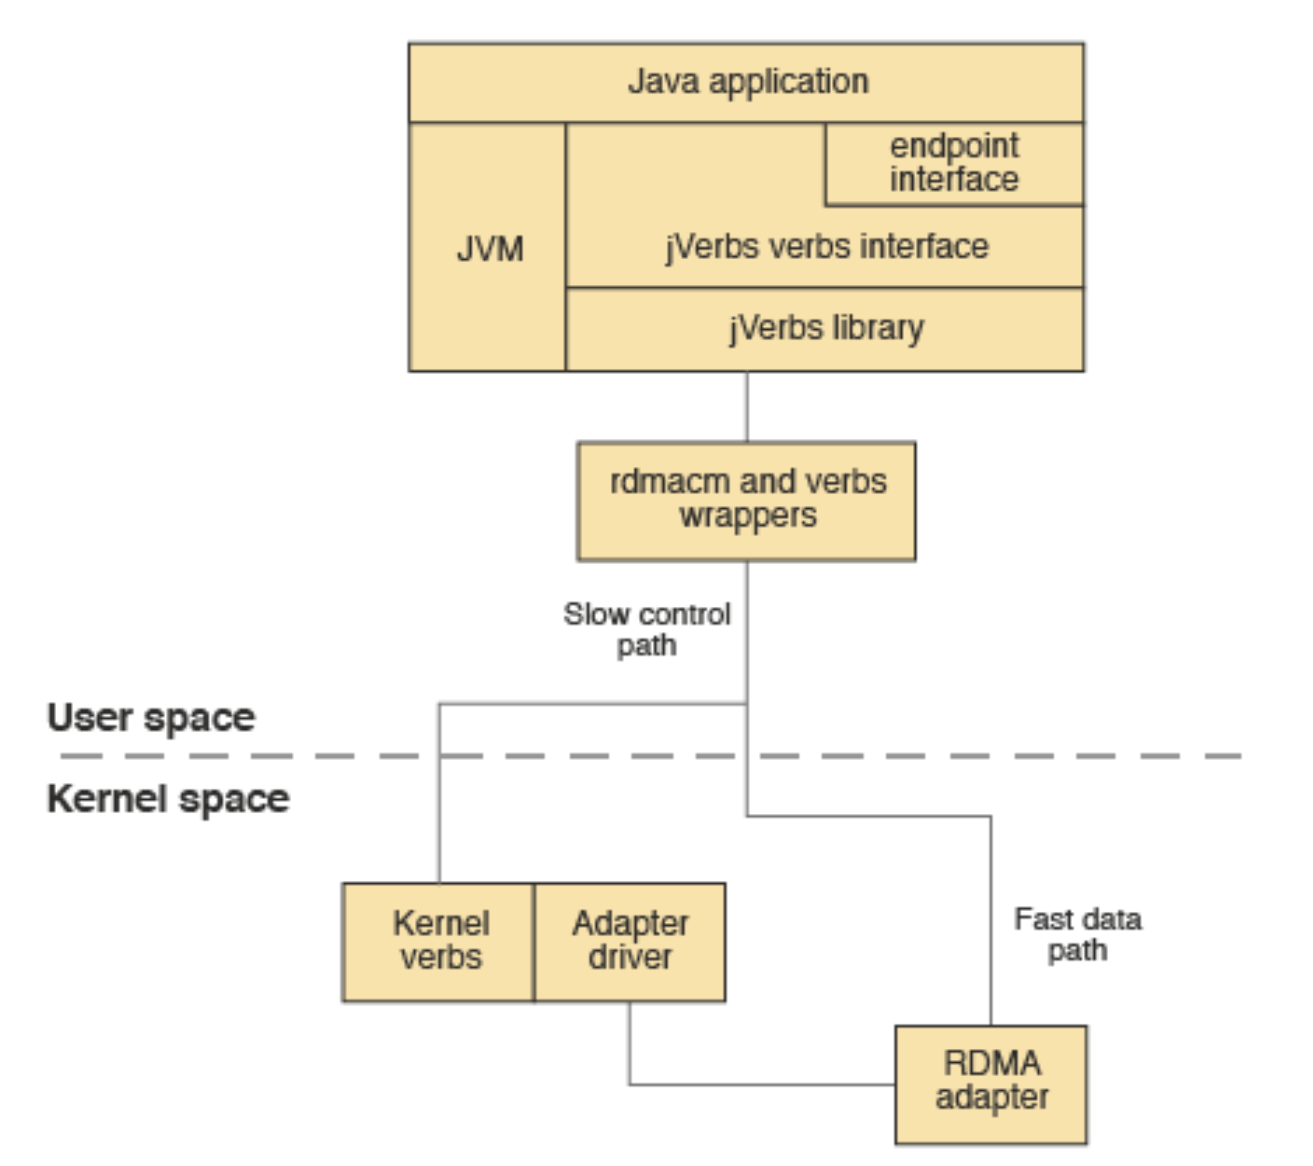
\includegraphics[width=\textwidth]{images/jverbs.png}
	\caption{jVerbs architecture - shows how the framework bypasses the kernel and JVM}
	\label{fig:jverb}
\end{figure}

jVerbs provides a useful example framework which re-emphasises that packet processing in Java is very possible with low latency, while assisting in certain implementation and design choices which can be analysed in more detail. 

\subsection{Native I/O API's}
\subsubsection{DPDK}
\subsubsection{Netmap}

\newpage

\section{Project Plan}
\subsection{Time Plan}
The given time plan outlined below provides me with a useful indication of how to measure the progress of the project, as well as dividing the whole project into smaller, more manageable sections which can be assessed individually. Some of the milestones have already been completed, while the others are expected to be finished within the given time period.
\subsubsection{Key Milestones}
\begin{itemize}
	\item Done - Background reading on DPDK \& Netmap
	\item Done - Understand workings off Java Native Interface (JNI) and Java memory
	\item Done - Get DPDK (and associated programs) working on local machine (or VM)
	\item In Progress - Link DPDK library with shared object files for JNI
	\item Awaiting - Implement basic IP address firewall
	\item Awaiting - Implement basic NAT
	\item Awaiting - Find similar implementations of firewall and NAT in C/C++ and Java
	\item Awaiting - Set up 2 independent machines to use for testing purposes
	\item Awaiting - Run tests on firewall and NAT to produces performance measurements
	\item Awaiting - Analyse results
\end{itemize}

\subsubsection{Time Estimations}
\begin{center}
	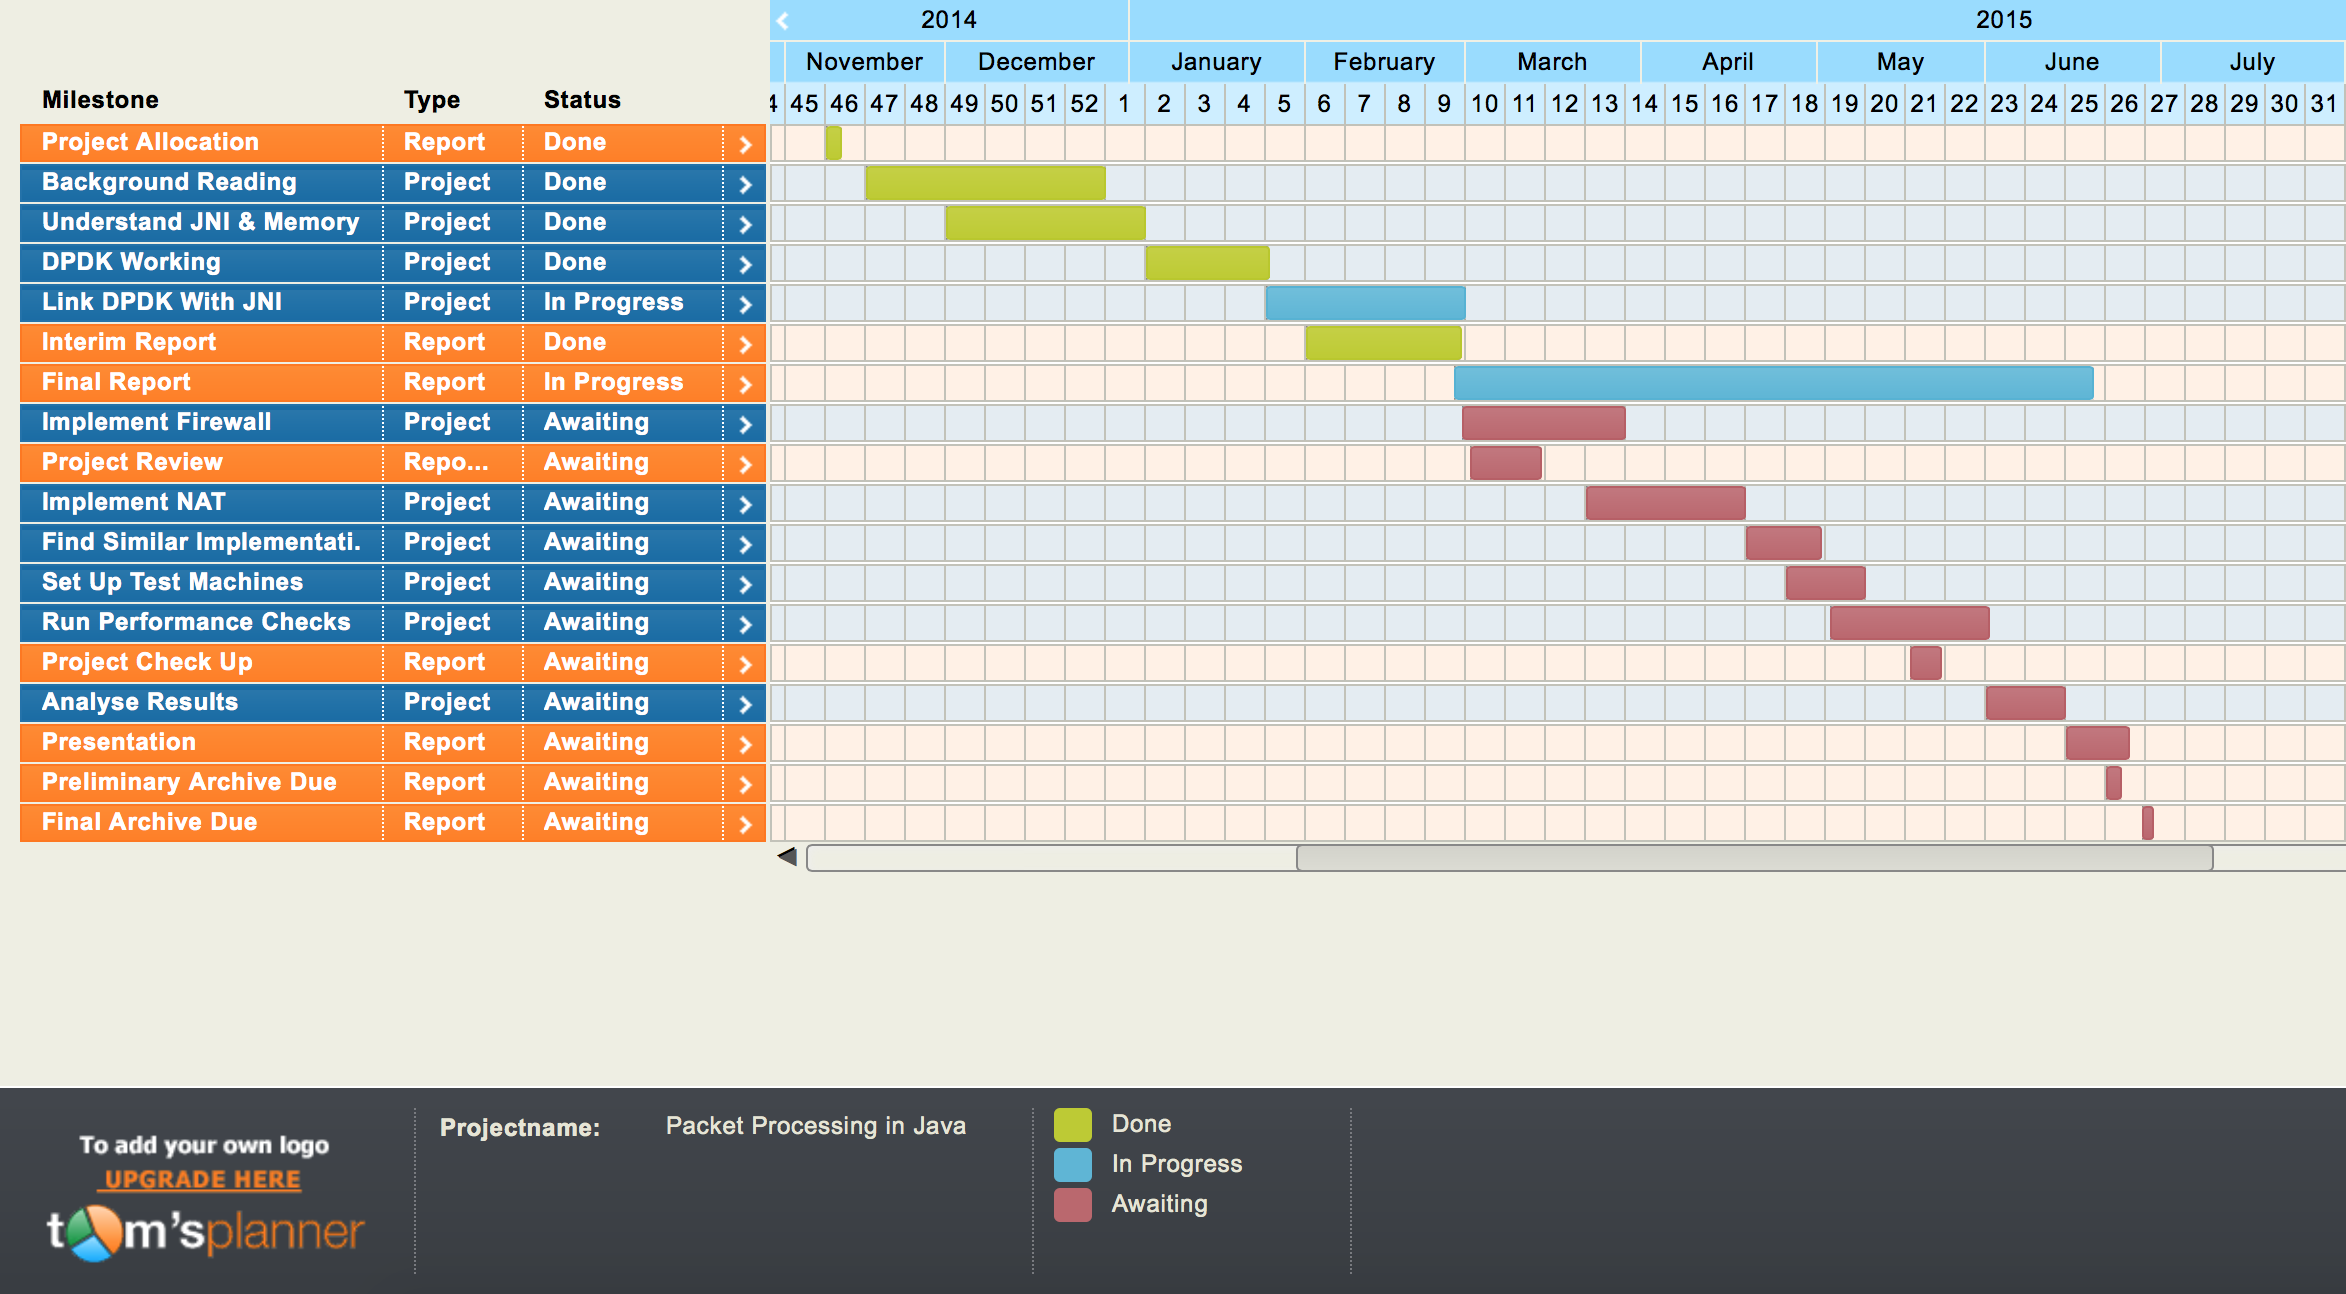
\includegraphics[width=\textwidth]{images/timeline.png}
\end{center}

\subsubsection{Completed Milestones}
As indicated, the background reading on the DPDK and Netmap libraries has been completed and the overview of the implementation has been assessed. The pros and cons has been outlined in the background section (give number). From this, I was able to get DPDK fully working on a virtual machine running locally on a personal machine, which allowed for a more in depth analysis of the implementation of DPDK. \\
\newline
I'm currently working on a way to generate shared object files from the C code used the link DPDK with a Java application. Due to the complex build system which DPDK makes use of, there has been a number of issues which have arisen.

\subsection{Fall Back Position}
If a number of unforeseen issues arise which impact on the progress of the project, I've outlined a few of the key milestones which can be omitted in order to allow the project to still be evaluated:
\begin{itemize}
	\item Implement basic NAT
	\item Find similar implementations of firewall and NAT in C/C++ and Java
	\item Run tests on firewall and NAT to produces performance measurements
\end{itemize}
Obviously, the emission of the above milestones will result in a less accurate evaluation of the overall project, but it's better than having nothing to evaluate in the end. As seen above, limiting the testing to one type of middlebox (only the firewall) can still give good results. This therefore reduces the need to look for an implementation for the NAT in Java and C/C++, while meaning less tests will have to be carried out. I feel that the remaining milestones are definitely key to the project in order for an adequate evaluation to be carried out.

\subsection{Possible Extensions}
If time allows, there are a number of possible extensions which can be undertaken to advance the project further forward and produce more data which can be evaluated later.

\subsubsection{Off Heap Java Memory}
In order for DPDK to handle packets correctly, it has to insert these packets onto the outgoing 'ring'. To do this, the Java application has to place its serialised objects into memory which DPDK can access. Under the current implementation, the Java application will directly place the packets onto the 'ring' using the direct ByteBuffer allocate feature. The other option is to use off heap java memory which DPDK can access and place onto the 'ring' automatically. This off heap memory is slightly slower than on heap memory but much faster than disk memory, while off heap memory stores object serialised and therefore ready for transmission in packets. \\
\newline
Altering the application to make use of off heap Java memory and then testing the results could potentially offer a new and faster way of high performance packet processing in Java.

\subsubsection{Limit Testing}
Another interesting extension could be to test the limitations of the NAT and firewall applications implemented within this project, and therefore limitations of the underlaying implementation. In terms of the project, the limitations could be on the max packet throughput which it can handle without having to buffer the incoming packets.

\newpage

\section{Evaluation Plan}
The sections below outline how the project will be evaluated in order to determine whether the initial objectives have been met and whether the final outcome can be deemed a success, even if it provides unexpected results.

\subsection{Experiments \& Outcomes}
The main measure of success will be from the experiments which are to be carried out. Using the high performance Java packet I/O application which is currently been developed as part of this project, it will be compared to similar, already existing applications written in pure Java and in C/C++. This comparison will consist of 2 parts, firstly an application for a NAT and secondly a simple IP address firewall. These similar applications will then be benchmarked against each other and the results analysed. \\
\newline
Benchmarking will consist of setting up 2 independent computers, most likely standalone machines, in order to take advantage of the ability to overwrite the Intel network card drivers as required by the DPDK API. Testing can the be carried out on the firewall and NAT implemented in the 3 different contexts, measuring the latency between the time sent and time received of the network packet. As the testing will be carried out on the same machines, linked to the same network there is unlikely to be much variation in the network latency. This means that the variation in the times will be from the system processing speeds. To account for minor variations in the computing performance of the system, numerous iterations of the same test will be carried out, then taking statistical averages will provide the best final results in order to analyse correctly. \\
\newline
Analysis of the results will be mainly carried out via the use of graphs which allow for easy comparison of results. The expected outcome is that the application developed from within this project is of similar speeds to applications coded directly in C/C++ and much faster than those coded in Java. This is mainly because the kernel will be bypassed, but the use of the Java Native Interface is expected to slow down certain aspects of the application. However, as long as speeds which coincide with those of the line rate are reached, this will be acceptable. There is the possibility that expected speeds are much faster than those that are actually measured. Although this isn't ideal, the project shouldn't be considered a failure as it will still provide very useful feedback as to where future investigations should be focussed on.

\subsection{Functionality \& Usability}
Although the objectives didn't specify any requirement to make the final application highly usable, my personal preference would be to have a product that could be used by anybody in the future. This obviously requires well commented and documented code. As the previous evaluation was all quantitative measurements, this evaluation will consist of qualitative measurements mainly undertaken by myself. \\
\newline
The functionality and usability can also be checked by the project supervisor \& co-supervisor to check if the original specifications were met. This can allow for an appraisal of the final application to be carried out which will be a good indication of the success of the project.

\newpage

\todo[inline]{Add references}
\todo[inline]{Add figure labels}
\todo[inline]{Do final read through}
\todo[inline]{Put through spell checker}
\todo[inline]{Other useful applications}
\todo[inline]{What font, size and line spacing?}
\todo[inline]{hyper link contents}
\todo[inline]{java network options don't allow for generic packets to be inspected}

\begin{thebibliography}{99}
%http://www.neclab.eu/Projects/midcom.htm \\
%http://windowsitpro.com/networking/what-types-network-address-translation-nat-exist \\
%http://en.wikipedia.org/wiki/Firewall_(computing)#mediaviewer/File:Firewall.png
\end{thebibliography}

\end{document}  